\subsubsection{Controlador Pixhawk}
O módulo Pixhawk piloto automático é um sistema muito eficiente em tempo real de operação. 
O software pode ser atualizado com um bootloader USB (gerenciador de boot USB), que é um programa simples com a 
função de acessar o disco do computador e carregar o sistema operacional na memória para assumir o controle do 
equipamento.

Os benefícios do sistema Pixhawk incluem \textit{multithreading}, ou seja, a capacidade de servir mais de um usuário ao 
mesmo tempo, um ambiente de programação Unix/Linux capaz de gerar novas funções de piloto automático, como 
escrita de missões e comportamento de voo. \cite{pix}
 
O módulo Pixhawk flagship pode ser utilizado visando as novas opções de periféricos, como sensor digital de velocidade do ar, o suporte para um indicador LED externo multicor e um magnetômetro externo. Todos os periféricos são automaticamente detectados e configurados. \cite{pix}

\subsubsection{Desfibrilador}

A escolha do desfibrilador, para ser carregado no VANT foi realizada visto que:

\begin{citacao}
foi documentada uma taxa de 
sobrevivência entre vítimas de parada cardíaca com fibrilação ventricular confirmada acima de 90\% quando a desfibrilação é atingida
dentro do primeiro minuto de colapso. As taxas de sobrevivência declinam 7 a 10\% a cada minuto em que a desfibrilação
é atrasada, de modo que uma vítima de parada cardíaca sem desfibrilação por 12 minutos tem apenas 2 a 5\%
de chance de sobrevivência.\cite{1}
\end{citacao}

O objetivo em realizar a Reanimação Cárdio-Pulmonar (RCP) é prover oxigênio ao cérebro e coração até que
o tratamento adequado restaure os batimentos cardíacos normais, ou que permita o tempo necessário para a 
chegada de uma equipe de socorro de Suporte Avançado de Vida (SAV). Quando o início da RCP for retardado, 
a chance de sobrevida é prejudicada e o córtex cerebral (o tecido mais susceptível à lesão por baixa de 
oxigênio no sangue) sofre danos irreversíveis,resultando em morte ou seqüelas neurológica severa e permanente. \cite{2}

O desfibrilador externo automático (DEA) por ser portátil e automático, torna a possível utilização por 
pessoas sem formação médica, visto que ele possui um computador embutido que verifica o ritmo cardíaco da 
pessoa e calcula se a desfibrilação se faz necessária, mostrando um comando para a pessoa acionar o botão, de 
modo a liberar a carga no peito da vitima.\cite{3}. O diagrama de bloco mostrado na Figura \ref{fig:dea}, mostra todo o funcionamento do DEA.

\begin{figure}[h!]
	\centering
	  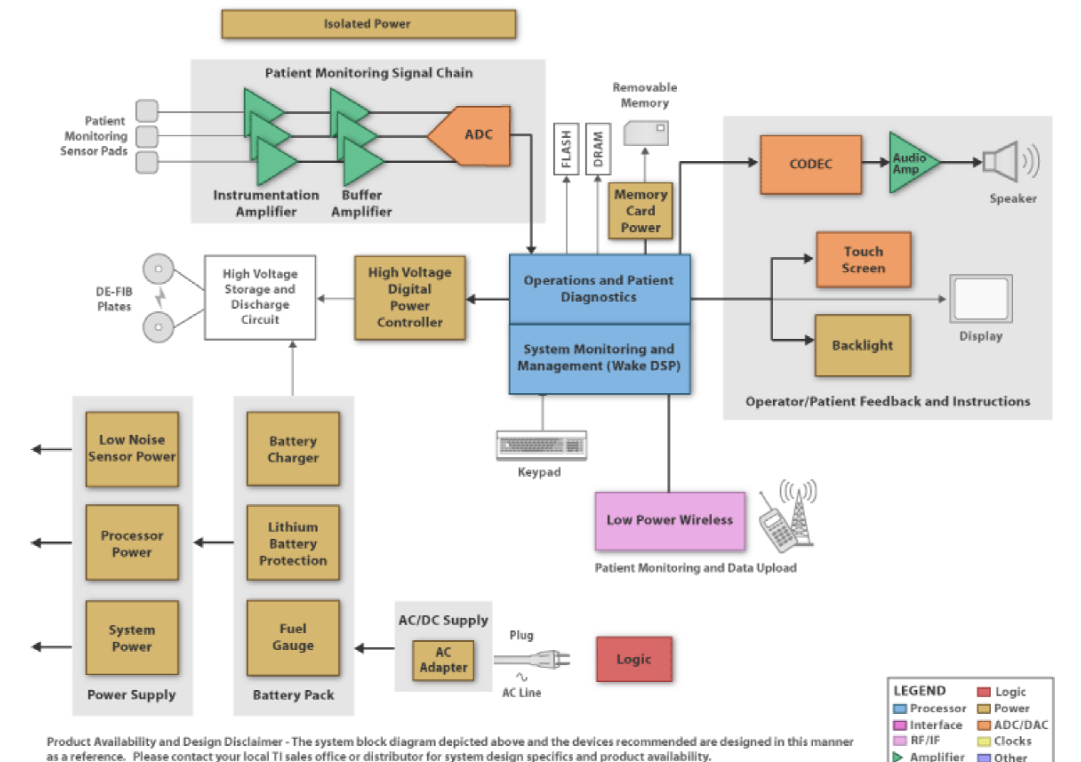
\includegraphics[keepaspectratio=true,scale=0.3]{figuras/dea.png}
	\caption{Diagrama de Bloco. Fonte: \cite{bloco}}
	\label{fig:dea}
\end{figure}

O desfibrilador, como demonstrado na Figura \ref{fig:dea}, consiste de uma fonte  de alimentação que 
fornece uma tensão regulada aos circuitos de controle e de interface do equipamento, além de fornecer uma carga.

A principal hipótese pela qual o choque elétrico desfibrilatório termina com a fibrilação ventricular (FV) se
baseia na despolarização de uma determinada massa crítica miocárdica, tornando-a temporariamente inexcitável, e
assim extinguindo as frentes de onda de excitação causadas pela manutenção da FV, de modo a permitir o 
restabelecimento do padrão normal de excitação e propagação elétrica (ZIPES et al., 1975 apud \citeonline{4}).

A figura \ref{fig:circuitodea} mostra todo o circuito eletrônico do DEA.

\begin{figure}[h!]
	\centering
		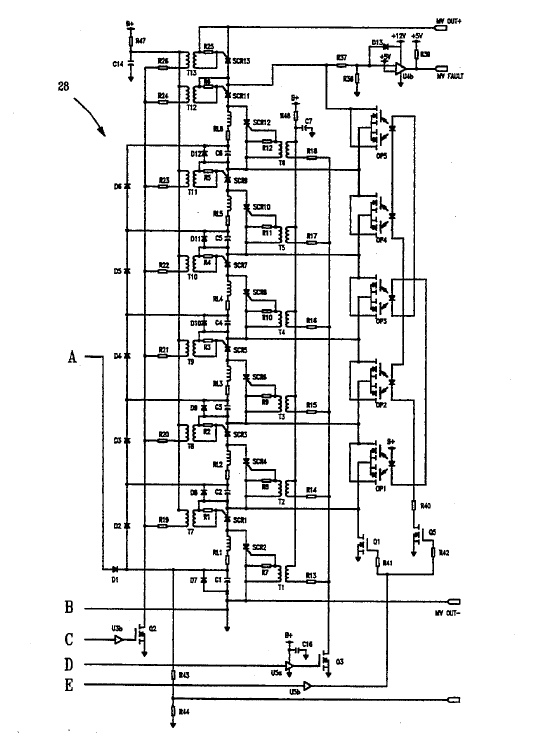
\includegraphics[keepaspectratio=true,scale=1.2,angle=-90]{figuras/circuitodea.png}
	\caption{Circuito eletrônico DEA. Fonte: \cite{dea}}
	\label{fig:circuitodea}
\end{figure}

\pagebreak
